The \ac{sm} of Particle Physics is the current theory that describes three of the four fundamental forces, namely the electromagnetic, strong, and weak forces, with the exception of gravity. Over the last decades it has been probed with remarkable precision but although there are  observational phenomena that lie beyond its scope. 

The SM is based on symmetry principles and is described by a lorentz-invariant \ac{qft}. This \ac{qft} is renormalizable and invariant under local gauge transformations belonging to the non-abelian gauge group 
\begin{equation}
    G = SU(3)_C \otimes SU(2)_L \otimes U(1)_Y,
\end{equation}
that leaves the equations of motions invariant under transformations within this group. $SU(3)_C$ is the special unitary group of rank 3 representing the color symmetry within \ac{qcd}, the \ac{qft} describing the strong interactions. $SU(2)_L \otimes U(1)_Y$ exhibits the unification of the weak and electromagnetic interaction into the electro-weak force of $SU(2)_L$ left-chiral fermions of the weak force and right-handed $U(1)_Y$ fermions with hypercharge $Y$ of the electromagnetic force described by Quantum Electrodynamics\ac{qed}. The following describes the particle content of the \ac{sm} and gives a brief overview of the \ac{qft}'s used to describe aforementioned forces. The content of this chapter draws inspiration primarily from \citep{hollik2010quantum,griffiths2020introduction,thomson2013modern}.


\section{Particle Content of the SM}

All currently known elementary particles are included in the \ac{sm} and can be organized as depicted in figure \ref{fig:sm}. This includes 12 fermions, that are particles of half-integer spin, 12 vector bosons with spin 1, and the Higgs boson, a scalar particle with spin 0. 


\begin{figure}
    \centering
    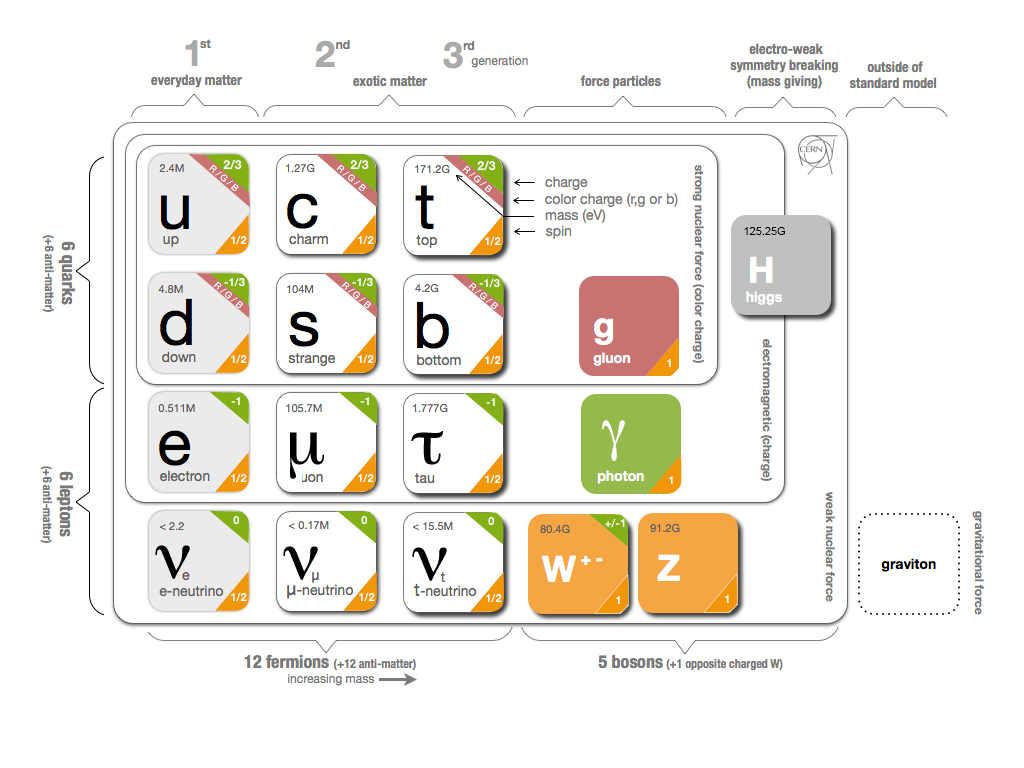
\includegraphics[width=1\textwidth]{SMinfographic_image_}
        \caption[]{Particles in the SM. Adopted from \citep{smpar}. Higgs Boson mass corrected to the current value \citep{particle2022review}. }
    \label{fig:sm}    
\end{figure}


The fermions can be categorized into three generations each consisting of a charged lepton, a neutral neutrino and two quarks. Except for their masses, particles of the different generations have the same quantum numbers. Ordinary matter consists only of particles from the first generation. Moreover each particle has an associated anti-particle with all the quantum numbers inversed. 

Quarks possess both electric charges and color charges, causing them to interact with each other via weak, electromagnetic, and strong forces. Each generation consists of an up quark (up, charm and top quark) with an electric charge of \mbox{Q = 2/3} and a down quark (down, strange and bottom quark) with a charge of \mbox{Q = -1/3}. Quarks can only be observed as composite particles - hadrons due to color confinement. This states that if one tries to separate a hadron, it is always energetically favorable to produce a quark-antiquark pair instead. Hadrons constitutes either bound states of 2 quarks - Mesons, e.g. a pion or 3 quarks - Baryons e.g. the proton. To not break Pauli's exclusion principle quarks in a bound state must have different color states.

Leptons in turn do not carry a color charge and encompasses the electron $e$, muon $\mu$ and tau $\tau$ and their associated neutrinos $\nu_e$, $\nu_\mu$ and $\nu_\tau$. In the \ac{sm} neutrinos are considered to be massless. Neutrinos also do not carry a charge and interact solely via the weak force whereas the  ones ($e$, $\mu$, $\tau$) with a charge $Q=-1$ participate also interact electromagnetically.

In the interaction picture of \ac{qft}, forces are mediated by particles specific to the particular force. These particles are bosons and are mediating as 8 massless gluons $g$ the strong force, as 1 massless photon $\gamma$ the electromagnetic force and as 3 massive bosons $W^+,W^-,Z$ the weak force. 

The scalar Higgs particle has a unique role in the Standard model. As will be explained in more detail in section \ref{sec:qed} a locally gauge free \ac{qft} requires a massless mediator which the $W^{\pm},Z$ are not. When unifying the weak force and the electromagnetic force into the electroweak force a new field - the Higgs field - can incorporate mass to these mediators by leaving the qft gaguge invariant. This will be discussed in detail in section \ref{sec:higgs_mechanism}. The Higgs field can explain the masses of all fermions as the coupling to each fermion is proportional to its mass. This essentially means that the heavier the particle, the stronger its interaction is with the Higgs field. 

If not further specified the following always includes the anti-particles when referred to a species or a particular particle.

\section{Quantum Electrodynamics}

\red{online fix link! }